\documentclass[10pt,aspectratio=169]{beamer}
\usepackage[T1]{fontenc}
\usepackage{lmodern}
\usepackage{graphicx}
\usepackage{booktabs}
\usepackage{amsmath,amssymb}
\usepackage{tikz}
\usetikzlibrary{arrows.meta,positioning,shapes.geometric}
\usepackage{listings}
\usepackage{xcolor}
\usepackage{hyperref}
\definecolor{Navy}{HTML}{14263E}
\definecolor{Ink}{HTML}{22354B}
\definecolor{Teal}{HTML}{068C91}
\definecolor{Coral}{HTML}{CD4F55}
\definecolor{Gold}{HTML}{E3A940}
\definecolor{Mist}{HTML}{EEF5F6}
\definecolor{Cloud}{HTML}{F4F7FA}
\definecolor{Steel}{HTML}{5C6F80}
\setbeamertemplate{navigation symbols}{}
\setbeamertemplate{headline}{}
\setbeamertemplate{frametitle}{%
 \nointerlineskip\begin{beamercolorbox}[wd=\paperwidth,ht=0.56cm,dp=0.17cm,leftskip=0.65cm]{frametitle}
 \usebeamerfont{frametitle}\insertframetitle\end{beamercolorbox}}
\setbeamercolor{normal text}{fg=Ink,bg=white}
\setbeamercolor{frametitle}{fg=white,bg=Navy}
\setbeamercolor{title}{fg=white}
\setbeamercolor{block title}{fg=white,bg=Teal}
\setbeamercolor{block body}{fg=Ink,bg=Mist}
\setbeamercolor{alertblock title}{fg=white,bg=Coral}
\setbeamercolor{alertblock body}{fg=Ink,bg=Cloud}
\setbeamercolor{exampleblock title}{fg=white,bg=Navy}
\setbeamercolor{exampleblock body}{fg=Ink,bg=Cloud}
\setbeamercolor{itemize item}{fg=Teal}
\setbeamercolor{itemize subitem}{fg=Teal}
\setbeamercolor{enumerate item}{fg=Teal}
\setbeamerfont{frametitle}{size=\large,series=\bfseries}
\setbeamerfont{block title}{series=\bfseries}
\setbeamercovered{invisible}
\setbeamertemplate{footline}{%
\leavevmode\hbox{\begin{beamercolorbox}[wd=.79\paperwidth,ht=.32cm,dp=.12cm,leftskip=.5cm]{normal text}\tiny\color{Steel}Python for Everyone (2/e) | Chapter 9: Objects and Classes \end{beamercolorbox}%
\begin{beamercolorbox}[wd=.21\paperwidth,ht=.32cm,dp=.12cm,rightskip=.5cm plus 1fil]{normal text}\hfill\tiny\color{Steel}\insertframenumber/\inserttotalframenumber\end{beamercolorbox}}}
\lstdefinestyle{py}{%
 language=Python,basicstyle=\ttfamily\fontsize{8.4}{10.7}\selectfont,
 keywordstyle=\bfseries\color{Teal},commentstyle=\itshape\color{Steel},stringstyle=\color{Coral},
 numbers=none,showstringspaces=false,columns=fullflexible,keepspaces=true,
 frame=single,framerule=.35pt,rulecolor=\color{Steel!30},
 backgroundcolor=\color{Cloud},xleftmargin=5pt,xrightmargin=5pt,
 aboveskip=6pt,belowskip=6pt,tabsize=4}
\lstset{style=py}
\newcommand{\imgcredit}[1]{{\par\vspace{2pt}\fontsize{6}{7}\selectfont\color{Steel}Source figure: Horstmann \& Necaise, \emph{Python for Everyone}, 2/e, p.~#1.}}
\newcommand{\prompt}[1]{\begin{block}{\texorpdfstring{\textbf{PREDICT / DISCUSS}}{PREDICT / DISCUSS}}#1\end{block}}
\newcommand{\reveal}[1]{\onslide<2->{\begin{alertblock}{Reveal and explain}#1\end{alertblock}}}
\newcommand{\step}[1]{\textcolor{Teal}{\bfseries #1}}
\newcommand{\smallfig}[2]{\includegraphics[width=#1]{ch09_assets/#2.pdf}}
\title{Chapter 9: Objects and Classes}
\subtitle{Interactive theory slides: Predict -- Trace -- Reveal -- Practice}
\author{Adapted for classroom instruction from \emph{Python for Everyone}, 2/e}
\date{}
\begin{document}

% 01
\begin{frame}[plain]
\begin{tikzpicture}[remember picture,overlay]
\fill[Navy] (current page.south west) rectangle (current page.north east);
\fill[Teal] ([xshift=-0.9cm]current page.north east) rectangle ([xshift=-0.72cm]current page.south east);
\node[anchor=west,text=white,align=left] at ([xshift=.9cm,yshift=.7cm]current page.west){\fontsize{28}{32}\selectfont\bfseries OBJECTS\quad\&\quad CLASSES\\[7pt]\fontsize{16}{19}\selectfont Chapter 9};
\node[anchor=west,text=white!75,align=left] at ([xshift=.9cm,yshift=-1.05cm]current page.west){\large Python for Everyone (2nd edition)\\[4pt]\small Interactive lecture | Theory + code tracing + quiz};
\node[anchor=south east] at ([xshift=-1.2cm,yshift=.7cm]current page.south east){\includegraphics[height=2.25cm]{ch09_assets/tally_counter.pdf}};
\end{tikzpicture}
\end{frame}

% 02
\begin{frame}{Learning outcomes}
By the end of this chapter, you should be able to:
\begin{enumerate}\setlength{\itemsep}{5pt}
\item Distinguish \textbf{class}, \textbf{object}, \textbf{method}, and \textbf{instance variable}.
\item Specify a class's \textbf{public interface} and explain \textbf{encapsulation}.
\item Implement \texttt{\_\_init\_\_}, methods, and \texttt{self} correctly.
\item Construct, trace, and unit-test multiple objects.
\item Explain \textbf{object references}, aliasing, \texttt{None}, and identity.
\item Design classes for simple applications (\texttt{CashRegister}, \texttt{BankAccount}, \texttt{Fraction}).
\end{enumerate}
\end{frame}

% 03
\begin{frame}{Chapter roadmap (textbook \S 9.1--9.11)}
\begin{columns}[T,onlytextwidth]
\column{.49\textwidth}
\begin{block}{I. What is an object?}
9.1 Object-oriented programming\\9.2 Implementing a simple class\\9.3 The public interface\\9.4 Data representation
\end{block}
\begin{block}{II. How is a class built?}
9.5 Constructors\\9.6 Implementing methods\\9.7 Testing a class
\end{block}
\column{.49\textwidth}
\begin{block}{III. How do objects behave?}
9.8 Tracing objects\\9.9 Patterns for object data\\9.10 Object references
\end{block}
\begin{block}{IV. Application}
9.11 Writing a \texttt{Fraction} class
\end{block}
\vspace{5pt}\small\textbf{Class routine:} predict the result \(\to\) run/trace \(\to\) explain. Press \(\rightarrow\) to reveal answers.
\end{columns}
\end{frame}

% 04
\begin{frame}{9.1 | From functions to objects}
\begin{columns}[T,onlytextwidth]
\column{.60\textwidth}
\begin{block}{Object-oriented programming (OOP)}
A program organizes its work around \textbf{objects} that combine:
\begin{itemize}
\item \textbf{State:} data belonging to the object;
\item \textbf{Behavior:} methods that use or change that state.
\end{itemize}
\end{block}
\begin{itemize}
\item A \textbf{class} defines a kind of object.
\item An \textbf{instance} is a particular object of that class.
\item Familiar objects: \texttt{str}, \texttt{list}, file handles.
\end{itemize}
\column{.37\textwidth}
\centering\smallfig{.95\linewidth}{tally_counter}
\imgcredit{502}
\small A \emph{Counter} class describes many independent tally counters.
\end{columns}
\end{frame}

% 05
\begin{frame}[fragile]{9.1 | Warm-up: methods belong to classes}
\prompt{Predict which expressions are valid Python method calls.}
\begin{lstlisting}
"Hello".upper()
["Hello", "World"].upper()
["Hello", "World"].pop()
"Hello".pop()
\end{lstlisting}
\reveal{\texttt{str} offers \texttt{upper()}, not \texttt{pop()}; \texttt{list} offers \texttt{pop()}, not \texttt{upper()}. A class determines its objects' available methods.}
\end{frame}

% 06
\begin{frame}{9.1 | Interface and encapsulation}
\begin{columns}[T,onlytextwidth]
\column{.51\textwidth}
\begin{block}{Public interface}
Methods that users of a class are meant to call, and the behavior these methods promise.
\end{block}
\begin{block}{Encapsulation}
Expose a useful interface while hiding internal data representation and implementation decisions.
\end{block}
\column{.46\textwidth}
\begin{exampleblock}{Think of a car}
You can steer and brake without learning how the engine works. Replacing the engine need not change how the driver uses the car.
\end{exampleblock}
\small\textbf{Discussion:} If a class changes from storing a total to storing individual items, must all its users change?
\onslide<2->{\small\step{No, provided the public methods retain their behavior.}}
\end{columns}
\end{frame}

% 07
\begin{frame}{9.2 | Our first class: \texttt{Counter}}
\begin{columns}[T,onlytextwidth]
\column{.60\textwidth}
The textbook begins with a \textbf{tally counter}: a click increases the displayed count.
\begin{block}{Required operations}
\texttt{click()} $\to$ increase the count by 1\\
\texttt{getValue()} $\to$ read the current count\\
\texttt{reset()} $\to$ set the count to 0
\end{block}
\small Each \texttt{Counter} needs its own stored value.
\column{.36\textwidth}
\centering\smallfig{.96\linewidth}{tally_counter}
\imgcredit{502}
\end{columns}
\end{frame}

% 08
\begin{frame}[fragile]{9.2 | Predict the tally counter's state}
\begin{lstlisting}
tally = Counter()
tally.reset()
tally.click()
tally.click()
result = tally.getValue()
tally.click()
print(result, tally.getValue())
\end{lstlisting}
\prompt{What does the last line print? Why do the two values differ?}
\reveal{Output: \texttt{2 3}. The integer in \texttt{result} stays \texttt{2}; the counter object itself remembers one more \texttt{click()}.}
\end{frame}

% 09
\begin{frame}{9.2 | Each instance has its own data}
\begin{columns}[T,onlytextwidth]
\column{.60\textwidth}
\centering\smallfig{\linewidth}{instance_variables}
\imgcredit{503, Fig.~2}
\column{.38\textwidth}
\begin{block}{Instance variables}
Storage locations associated with \emph{each object} of a class.
\end{block}
\small\texttt{concertCounter.\_value} and \texttt{boardingCounter.\_value} are \textbf{distinct} state variables.
\vspace{8pt}\small A leading underscore signals an implementation detail by convention; Python does not enforce strict privacy.
\end{columns}
\end{frame}

% 10
\begin{frame}[fragile]{9.2 | Original \texttt{Counter} implementation}
\begin{columns}[T,onlytextwidth]
\column{.58\textwidth}
\begin{lstlisting}
class Counter :
    def getValue(self) :
        return self._value

    def click(self) :
        self._value = self._value + 1

    def reset(self) :
        self._value = 0
\end{lstlisting}
\column{.39\textwidth}
\begin{itemize}
\item \texttt{self.\_value} means this object's value.
\item \texttt{getValue} is an \textbf{accessor}.
\item \texttt{click} and \texttt{reset} are \textbf{mutators}.
\item The book initially initializes the value by calling \texttt{reset()}.
\end{itemize}
\end{columns}
\end{frame}

% 11
\begin{frame}[fragile]{9.2 | Find the bug (textbook Self Check 5)}
\begin{lstlisting}
tally = Counter()
tally.click()
print(tally.getValue())
\end{lstlisting}
\prompt{With the \emph{original} Counter implementation, does this work?}
\reveal{\textbf{No.} \texttt{\_value} has not been created; \texttt{click()} tries to read it and raises an \texttt{AttributeError}. Section 9.5 fixes the design using a constructor.}
\end{frame}

% 12
\begin{frame}{9.3 | Design the interface first: \texttt{CashRegister}}
\begin{columns}[T,onlytextwidth]
\column{.60\textwidth}
\begin{block}{Cash register responsibilities}
\begin{itemize}
\item \texttt{addItem(price)} -- record an item;
\item \texttt{getTotal()} -- return the amount owed;
\item \texttt{getCount()} -- return the number of items;
\item \texttt{clear()} -- start a new sale.
\end{itemize}
\end{block}
Start by deciding what the object should \emph{do}; choose data storage later.
\column{.36\textwidth}
\centering\smallfig{.97\linewidth}{register_photo}\imgcredit{506}
\end{columns}
\end{frame}

% 13
\begin{frame}{9.3 | Mutator or accessor?}
\prompt{For \texttt{CashRegister}, classify each method and justify your choice.}
\begin{center}
\begin{tabular}{lc}
\toprule\textbf{Method}&\textbf{Classification}\\\midrule
\texttt{addItem(price)} & \onslide<2->{Mutator}\\[5pt]
\texttt{getTotal()} & \onslide<2->{Accessor}\\[5pt]
\texttt{getCount()} & \onslide<2->{Accessor}\\[5pt]
\texttt{clear()} & \onslide<2->{Mutator}\\\bottomrule
\end{tabular}
\end{center}
\onslide<2->{\small\textbf{Mutator:} changes object state. \textbf{Accessor:} reports information without changing it.}
\end{frame}

% 14
\begin{frame}[fragile]{9.3 | Construct, reference, call}
\begin{columns}[T,onlytextwidth]
\column{.53\textwidth}
\begin{lstlisting}
register1 = CashRegister()
register1.addItem(1.95)
print(register1.getTotal())
\end{lstlisting}
\begin{itemize}
\item \texttt{CashRegister()} creates an object.
\item \texttt{register1} refers to that object.
\item \texttt{register1.addItem(...)} sends it a method call.
\end{itemize}
\column{.44\textwidth}
\centering\smallfig{\linewidth}{cashregister_reference}
\imgcredit{507, Fig.~3}
\end{columns}
\end{frame}

% 15
\begin{frame}{9.4 | Choose the data representation}
Two possible internal designs for the \emph{same} public interface:
\vspace{5pt}
\begin{columns}[T,onlytextwidth]
\column{.48\textwidth}
\begin{block}{A. Store every item}
\texttt{\_prices = [1.95, 0.95, 2.50]}\\
\texttt{getTotal(): sum(\_prices)}\\
\texttt{getCount(): len(\_prices)}
\end{block}
\column{.48\textwidth}
\begin{block}{B. Store summary statistics}
\texttt{\_totalPrice = 5.40}\\
\texttt{\_itemCount = 3}\\
\texttt{getTotal(): \_totalPrice}
\end{block}
\end{columns}
\vspace{6pt}\small The textbook chooses design \textbf{B}: simple, constant-time updates and queries for this interface.
\end{frame}

% 16
\begin{frame}{9.4 | A design question}
\prompt{Suppose a future method \texttt{removeLastItem()} must undo the most recent item. Which representation is more convenient?}
\begin{enumerate}[A.]
\item Store only \texttt{\_totalPrice} and \texttt{\_itemCount}.
\item Store the list of added prices.
\item Both are equally convenient without extra state.
\end{enumerate}
\reveal{\textbf{B.} The list retains item-level history. This illustrates that representation should support the \emph{required} behavior, not simply use the smallest number of variables.}
\end{frame}

% 17
\begin{frame}[fragile]{9.5 | Constructors: initialize state}
\begin{columns}[T,onlytextwidth]
\column{.52\textwidth}
\begin{lstlisting}
class CashRegister :
    def __init__(self) :
        self._itemCount = 0
        self._totalPrice = 0.0

reg = CashRegister()
\end{lstlisting}
\begin{itemize}
\item \texttt{\_\_init\_\_} runs during construction.
\item It establishes instance variables before other methods run.
\item \texttt{self} refers to the new object.
\end{itemize}
\column{.45\textwidth}
\centering\smallfig{\linewidth}{constructor_syntax}
\imgcredit{511, Syntax 9.1}
\end{columns}
\end{frame}

% 18
\begin{frame}[fragile]{9.5 | Constructor with an argument}
\begin{lstlisting}
class BankAccount :
    def __init__(self, initialBalance = 0.0) :
        self._balance = initialBalance

account1 = BankAccount()
account2 = BankAccount(1000.0)
account3 = BankAccount(initialBalance = 25.0)
\end{lstlisting}
\begin{block}{Key distinction}
\texttt{BankAccount(...)} is the construction expression. The special method \texttt{\_\_init\_\_} initializes the newly created instance; in normal code you do \textbf{not} call it explicitly to make a new object.
\end{block}
\end{frame}

% 19
\begin{frame}[fragile]{9.5 | Choose the correct construction syntax}
\prompt{Which expression creates a separate \texttt{BankAccount} object with initial balance 250?}
\begin{lstlisting}
A: BankAccount.__init__(250)
B: BankAccount(250)
C: BankAccount()._balance = 250
D: BankAccount.__init__(self, 250)
\end{lstlisting}
\reveal{\textbf{B.} A and D misuse \texttt{\_\_init\_\_}; C assigns to internal state and is not the intended construction expression.}
\end{frame}

% 20
\begin{frame}[fragile]{9.6 | What does \texttt{self} mean?}
\begin{lstlisting}
class CashRegister :
    def addItem(self, price) :
        self._itemCount += 1
        self._totalPrice += price

register1.addItem(2.95)
\end{lstlisting}
\begin{block}{Behind the notation}
On this method call, \texttt{self} is bound to the object referenced by \texttt{register1}; \texttt{price} receives \texttt{2.95}. The caller does not supply \texttt{self} as an explicit argument.
\end{block}
\end{frame}

% 21
\begin{frame}{9.6 | Trace the method call visually (textbook Fig. 4)}
\centering
\only<1>{\textbf{Step 1: Before calling \texttt{register1.addItem(2.95)}}\\[7pt]
\includegraphics[width=.82\linewidth]{ch09_assets/self_before_clean.pdf}\\[8pt]
\small The register exists and its state is initialized to zero.}
\only<2>{\textbf{Step 2: During the method call}\\[7pt]
\includegraphics[width=.82\linewidth]{ch09_assets/self_during_clean.pdf}\\[8pt]
\small The temporary \texttt{self} reference points to \texttt{register1}; \texttt{price = 2.95}.}
\only<3>{\textbf{Step 3: After the method call}\\[7pt]
\includegraphics[width=.82\linewidth]{ch09_assets/self_after_clean.pdf}\\[8pt]
\small The item count becomes 1 and the total price becomes 2.95.}
\vspace{10pt}\imgcredit{513--514, Fig.~4}
\end{frame}

% 22
\begin{frame}[fragile]{9.6 | Complete \texttt{CashRegister} (part 1)}
\begin{lstlisting}
class CashRegister :
    def __init__(self) :
        self._itemCount = 0
        self._totalPrice = 0.0

    def addItem(self, price) :
        self._itemCount += 1
        self._totalPrice += price

    def getTotal(self) :
        return self._totalPrice
\end{lstlisting}
\small Each method reads or changes the state of the \emph{current} register through \texttt{self}.
\end{frame}

% 23
\begin{frame}[fragile]{9.6 | Complete \texttt{CashRegister} (part 2)}
\begin{lstlisting}
    def getCount(self) :
        return self._itemCount

    def clear(self) :
        self._itemCount = 0
        self._totalPrice = 0.0
\end{lstlisting}
\begin{block}{Design convention from the chapter}
Create instance variables in \texttt{\_\_init\_\_}. Use public methods to change/query them. The leading underscore marks implementation details, even though Python permits access.
\end{block}
\end{frame}

% 24
\begin{frame}[fragile]{9.6 | Interactive trace: two objects}
\begin{lstlisting}
a = CashRegister()
b = CashRegister()
a.addItem(1.95)
a.addItem(0.95)
b.addItem(5.00)
print(a.getCount(), a.getTotal())
print(b.getCount(), b.getTotal())
\end{lstlisting}
\prompt{Predict the two printed lines. Is \texttt{b} affected by operations on \texttt{a}?}
\reveal{\texttt{2 2.9} and \texttt{1 5.0}. Each constructed object has separate instance variables. For currency display, use \texttt{\%.2f} formatting.}
\end{frame}

% 25
\begin{frame}{9.6 | Optional: class variables vs instance variables}
\begin{columns}[T,onlytextwidth]
\column{.51\textwidth}
\begin{block}{Instance variable}
\texttt{self.\_balance}: one value per account
\end{block}
\begin{block}{Class variable}
\texttt{BankAccount.\_lastAssignedNumber}: one shared value used to give sequential account numbers
\end{block}
\column{.46\textwidth}
\centering
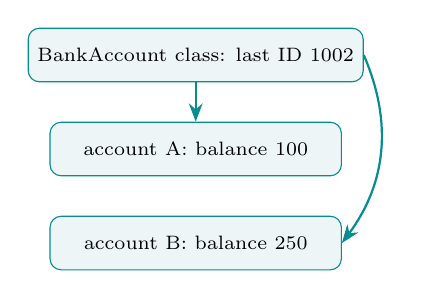
\begin{tikzpicture}[node distance=5mm, every node/.style={font=\scriptsize}, box/.style={draw=Teal,rounded corners,fill=Mist,minimum width=3.7cm,minimum height=0.68cm}]
\node[box] (cls) {BankAccount class: last ID 1002};
\node[box,below=of cls] (a) {account A: balance 100};
\node[box,below=of a] (b) {account B: balance 250};
\draw[-{Stealth},thick,Teal] (cls) -- (a);\draw[-{Stealth},thick,Teal] (cls.east) to[bend left=30] (b.east);
\end{tikzpicture}
\end{columns}
\end{frame}

% 26
\begin{frame}{9.7 | Unit testing a class}
\begin{block}{Unit test = isolated verification}
Construct objects, call methods, compare results against known expectations. Repeat tests after any code change.
\end{block}
\begin{enumerate}\setlength{\itemsep}{3pt}
\item Start with the initial state.
\item Exercise each public method.
\item Test sequences of mutator calls.
\item Test multiple independent objects.
\item Include boundary/error cases where relevant.
\end{enumerate}
\small The textbook demonstrates testing \texttt{CashRegister} in the Python shell and through a separate tester program.
\end{frame}

% 27
\begin{frame}[fragile]{9.7 | A tiny test driver with \texttt{assert}}
\begin{lstlisting}
reg = CashRegister()
assert reg.getTotal() == 0.0
assert reg.getCount() == 0

reg.addItem(1.95)
reg.addItem(0.95)
reg.addItem(2.50)
assert reg.getCount() == 3
assert abs(reg.getTotal() - 5.40) < 1e-9

reg.clear()
assert reg.getCount() == 0
\end{lstlisting}
\small\textbf{Why tolerance?} Floating-point totals may not be represented exactly; \texttt{assert} also makes the expected result explicit.
\end{frame}

% 28
\begin{frame}[fragile]{9.7 | Debugging challenge}
A programmer accidentally writes:
\begin{lstlisting}
def addItem(self, price) :
    self._itemCount += 1
    self._totalPrice = price
\end{lstlisting}
\prompt{Which unit test reveals the error? What correction is needed?}
\reveal{Add at least \textbf{two} items, then test the total. The assignment replaces the prior total. Correct it to \texttt{self.\_totalPrice += price}. A one-item test would miss this bug.}
\end{frame}

% 29
\begin{frame}{9.7 | How To 9.1: implement a class systematically}
\begin{columns}[T,onlytextwidth]
\column{.52\textwidth}
\begin{enumerate}\setlength{\itemsep}{6pt}
\item Identify object responsibilities.
\item Specify and document the public interface.
\item Determine instance variables and invariants.
\item Implement constructors and methods.
\item Test with representative and edge cases.
\end{enumerate}
\column{.45\textwidth}
\begin{exampleblock}{Worked example: BankAccount}
The book applies this process to deposits, withdrawals, overdraft penalties, interest and balance reporting.
\end{exampleblock}
\end{columns}
\end{frame}

% 30
\begin{frame}{Worked Example 9.1 | Design a bank account}
\begin{columns}[T,onlytextwidth]
\column{.60\textwidth}
\textbf{Problem rules (from the textbook):}
\begin{itemize}\setlength{\itemsep}{5pt}
\item Deposit increases the balance.
\item Withdrawal decreases the balance if sufficient funds exist.
\item Otherwise charge a fixed \textbf{\$10} penalty.
\item Monthly interest rate is passed to a method.
\item Current balance can be queried.
\end{itemize}
\column{.36\textwidth}
\begin{block}{Public methods}
\texttt{deposit(amount)}\\
\texttt{withdraw(amount)}\\
\texttt{addInterest(rate)}\\
\texttt{getBalance()}
\end{block}
\end{columns}
\end{frame}

% 31
\begin{frame}[fragile]{Worked Example 9.1 | \texttt{BankAccount} code}
\begin{lstlisting}
class BankAccount :
    def __init__(self, initialBalance = 0.0) :
        self._balance = initialBalance

    def deposit(self, amount) :
        self._balance += amount

    def withdraw(self, amount) :
        if amount > self._balance :
            self._balance -= 10.0
        else :
            self._balance -= amount
\end{lstlisting}
\small\textbf{Discussion:} Is the insufficient-funds branch rejecting a withdrawal or allowing overdraft? \onslide<2->{\step{It does not withdraw the requested amount; it charges only the penalty.}}
\end{frame}

% 32
\begin{frame}[fragile]{Worked Example 9.1 | Interest and testing}
\begin{lstlisting}
    def addInterest(self, rate) :
        self._balance += self._balance * rate / 100.0
    def getBalance(self) :
        return self._balance
acc = BankAccount(1000.0)
acc.deposit(500.0)
acc.withdraw(2000.0)
acc.addInterest(1.0)
print("%.2f" % acc.getBalance())
\end{lstlisting}
\prompt{Predict the final balance. Show the state after every call.}
\reveal{\(1000 \to 1500 \to 1490 \to 1504.90\). Output: \texttt{1504.90} (textbook p.~524).}
\end{frame}

% 33
\begin{frame}{9.8 | Tracing an object's state}
\begin{columns}[T,onlytextwidth]
\column{.53\textwidth}
\begin{itemize}\setlength{\itemsep}{7pt}
\item Write the object's public methods on a card.
\item Track instance variables on the back.
\item Execute mutators \textbf{one call at a time}.
\item Read accessors without changing state.
\end{itemize}
\column{.45\textwidth}
\centering\smallfig{\linewidth}{tracing_front}
\imgcredit{525, tracing cards}
\end{columns}
\end{frame}

% 34
\begin{frame}[fragile]{9.8 | Complete a state trace}
\begin{columns}[T,onlytextwidth]
\column{.55\textwidth}
\begin{lstlisting}
reg = CashRegister()
reg.addItem(19.95)
reg.addItem(2.05)
reg.clear()
reg.addItem(3.00)
\end{lstlisting}
\column{.41\textwidth}
\small\begin{tabular}{lcc}
\toprule Step & Count & Total\\\midrule
Construct & 0 & 0.00\\
\texttt{addItem(19.95)} & \onslide<2->{1} & \onslide<2->{19.95}\\
\texttt{addItem(2.05)} & \onslide<2->{2} & \onslide<2->{22.00}\\
\texttt{clear()} & \onslide<2->{0} & \onslide<2->{0.00}\\
\texttt{addItem(3.00)} & \onslide<2->{1} & \onslide<2->{3.00}\\\bottomrule
\end{tabular}
\end{columns}
\vspace{5pt}\small\textbf{Practice:} How would you test this sequence automatically?
\end{frame}

% 35
\begin{frame}{9.9 | Recurring patterns for object data}
\small\begin{tabular}{p{.29\linewidth}p{.58\linewidth}}
\toprule\textbf{Pattern}&\textbf{Example from the chapter}\\\midrule
Keeping a total & Cash register accumulated price; bank account balance\\[3pt]
Counting events & Number of added items; tally counter clicks\\[3pt]
Collecting values & A shopping cart or collection of items\\[3pt]
Managing properties & A product with mutable name/price properties\\[3pt]
Distinct states & A device that is on/off or in modes\\[3pt]
Position in space & Objects with coordinates / direction\\\bottomrule
\end{tabular}
\vspace{8pt}\small Ask: \emph{What must this object remember to support all its methods?}
\end{frame}

% 36
\begin{frame}{9.9 | Which state pattern should you use?}
\prompt{Match each new feature with a useful data representation.}
\begin{enumerate}
\item Record how many customers entered a store.
\item Undo the last three items purchased.
\item Store a device's operating mode (\texttt{OFF}, \texttt{READY}, \texttt{RUNNING}).
\end{enumerate}
\reveal{\textbf{1.} Event counter; \textbf{2.} Collection/stack of item prices; \textbf{3.} Distinct state variable with well-defined transitions.}
\end{frame}

% 37
\begin{frame}{9.10 | A variable refers to an object}
\begin{columns}[T,onlytextwidth]
\column{.48\textwidth}
\centering\smallfig{\linewidth}{one_reference}
\imgcredit{534, Fig.~5}
\column{.49\textwidth}
\begin{block}{Object reference}
A variable such as \texttt{reg1} holds a reference to an object, not an independent copy of all its internal data.
\end{block}
\texttt{reg1 = CashRegister()} binds a name to a newly constructed instance.
\end{columns}
\end{frame}

% 38
\begin{frame}[fragile]{9.10 | Shared references (aliasing)}
\begin{columns}[T,onlytextwidth]
\column{.50\textwidth}
\begin{lstlisting}
reg1 = CashRegister()
reg2 = reg1
reg2.addItem(2.95)
print(reg1.getTotal())
\end{lstlisting}
\prompt{What does the last line print?}
\onslide<2->{\small\textbf{Answer:} \texttt{2.95}. Both names refer to the \emph{same} object.}
\column{.47\textwidth}
\centering\smallfig{\linewidth}{shared_reference}
\imgcredit{534, Fig.~6}
\end{columns}
\end{frame}

% 39
\begin{frame}{9.10 | Copying references: textbook Fig. 7}
\begin{columns}[T,onlytextwidth]
\column{.53\textwidth}
\centering\includegraphics[height=.70\textheight]{ch09_assets/copy_references.pdf}
\imgcredit{535, Fig.~7}
\column{.44\textwidth}
\begin{enumerate}\setlength{\itemsep}{9pt}
\item Create a register.
\item Assign its reference to another name.
\item Update through the second name.
\end{enumerate}
\small\textbf{Important:} Assignment of a reference does \emph{not} make a copy of the object.
\end{columns}
\end{frame}

% 40
\begin{frame}[fragile]{9.10 | \texttt{is} versus \texttt{==}}
\begin{lstlisting}
a = CashRegister()
b = a
c = CashRegister()
print(a is b)
print(a is c)
\end{lstlisting}
\prompt{Predict both outputs. Which operation tests object identity?}
\reveal{Output: \texttt{True}, \texttt{False}. \texttt{is} tests identity: whether two references denote the same object. \texttt{==} tests equality according to the class's implementation (by default, ordinary user-defined instances compare by identity).}
\end{frame}

% 41
\begin{frame}[fragile]{9.10 | \texttt{None} and the special \texttt{self} reference}
\begin{columns}[T,onlytextwidth]
\column{.54\textwidth}
\begin{lstlisting}
reg = None
if reg is None :
    reg = CashRegister()

reg.addItem(2.95)
\end{lstlisting}
\begin{itemize}
\item \texttt{None} represents no object reference.
\item Use \texttt{is None}, not method calls on \texttt{None}.
\item While a method executes, \texttt{self} refers to its receiver object.
\end{itemize}
\column{.43\textwidth}
\centering\smallfig{\linewidth}{self_reference}
\imgcredit{536, Fig.~8}
\end{columns}
\end{frame}

% 42
\begin{frame}{9.11 | Application: rational numbers}
\begin{columns}[T,onlytextwidth]
\column{.59\textwidth}
\begin{block}{Motivation}
A \texttt{Fraction} object represents a rational number using \textbf{two integers}, reducing the roundoff issues that arise in floating-point arithmetic.
\end{block}
\begin{itemize}
\item Store \texttt{\_numerator} and \texttt{\_denominator}.
\item Denominator must be nonzero.
\item Normalize sign and reduce to lowest terms.
\item Keep objects \textbf{immutable} (as designed in the book).
\end{itemize}
\column{.37\textwidth}
\centering\smallfig{\linewidth}{fraction_photo}
\imgcredit{538}
\end{columns}
\end{frame}

% 43
\begin{frame}[fragile]{9.11 | Constructor invariant: canonical form}
\begin{lstlisting}
from math import gcd
class Fraction :
    def __init__(self, numerator=0, denominator=1) :
        if denominator == 0 :
            raise ZeroDivisionError("Zero denominator")
        if denominator < 0 :
            numerator, denominator = -numerator, -denominator
        d = gcd(abs(numerator), denominator)
        self._numerator = numerator // d
        self._denominator = denominator // d
\end{lstlisting}
\small\textbf{Textbook connection:} the book implements the GCD calculation with Euclid's algorithm directly. The \texttt{math.gcd} call here is an equivalent modern shortcut.
\end{frame}

% 44
\begin{frame}[fragile]{9.11 | Predict normalized fractions}
\begin{lstlisting}
f1 = Fraction(-2, -4)
f2 = Fraction(0, 15)
f3 = Fraction(3, -7)
f4 = Fraction(8, 0)
\end{lstlisting}
\prompt{What \texttt{(numerator, denominator)} pair is stored in each case? What happens for \texttt{f4}?}
\reveal{\texttt{f1: (1,2)}, \texttt{f2: (0,1)}, \texttt{f3: (-3,7)}. Constructing \texttt{f4} raises \texttt{ZeroDivisionError}. These are the normalization rules used by the book.}
\end{frame}

% 45
\begin{frame}[fragile]{9.11 | Add fractions without floating-point arithmetic}
\begin{lstlisting}
class Fraction :
    # ... constructor and other methods ...
    def __add__(self, other) :
        n = (self._numerator * other._denominator
             + other._numerator * self._denominator)
        d = self._denominator * other._denominator
        return Fraction(n, d)
\end{lstlisting}
\prompt{Predict \texttt{Fraction(1, 6) + Fraction(1, 3)}. What is the returned object's state?}
\reveal{\(\frac16 + \frac13 = \frac36 = \frac12\). The new object stores \texttt{(1,2)}. The operands remain unchanged; \texttt{\_\_add\_\_} creates a fresh \texttt{Fraction}.}
\end{frame}

% 46
\begin{frame}{9.11 | Special methods for numeric objects}
\small\begin{tabular}{p{.22\linewidth}p{.31\linewidth}p{.38\linewidth}}
\toprule\textbf{Method}&\textbf{Syntax used by caller}&\textbf{Purpose}\\\midrule
\texttt{\_\_str\_\_} & \texttt{print(f)} & Human-readable representation\\[4pt]
\texttt{\_\_add\_\_} & \texttt{f1 + f2} & Add fractions; return a new object\\[4pt]
\texttt{\_\_eq\_\_} & \texttt{f1 == f2} & Value-based equality check\\[4pt]
\texttt{\_\_lt\_\_} & \texttt{f1 < f2} & Less-than comparison\\\bottomrule
\end{tabular}
\vspace{5pt}\small The textbook covers arithmetic and logical operations in its \texttt{Fraction} application. Operator overloading supports familiar syntax.
\end{frame}

% 47
\begin{frame}{Concept check | 6 essentials}
\prompt{Without looking back, answer the following:}
\begin{enumerate}\setlength{\itemsep}{4pt}
\item What is the difference between a class and an object?
\item Why hide instance variables behind public methods?
\item What is the role of \texttt{\_\_init\_\_}?
\item What does \texttt{self} refer to during a method call?
\item Why can two names change the same object?
\item What are the goals of a class-level unit test?
\end{enumerate}
\onslide<2->{\small\textbf{Instructor discussion:} definition/template vs instance; encapsulation; initialization; receiver; aliasing; reliable behavior and regression checks.}
\end{frame}

% 48
\begin{frame}[fragile]{Mini-lab 1 | Repair and extend \texttt{Counter}}
\begin{lstlisting}
class Counter :
    def __init__(self, start=0) :
        self._value = start

    def click(self) :
        # TODO: add one to the stored value
        pass

    def getValue(self) :
        # TODO: return the stored value
        pass
\end{lstlisting}
\small\textbf{Tasks:} (1) fill in the two bodies; (2) implement \texttt{reset()}; (3) test two counters with different starts; (4) use \texttt{assert} to verify independence.
\end{frame}

% 49
\begin{frame}[fragile]{Mini-lab 2 | Extend \texttt{CashRegister}}
\textbf{Requirements:} implement \texttt{giveChange(self, payment)} such that it returns the change and clears the register for the next sale (the textbook's Self Check 27).
\begin{lstlisting}
def giveChange(self, payment) :
    # TODO: compute change from _totalPrice
    # TODO: clear the current sale
    # TODO: return the change
    pass
\end{lstlisting}
\small\textbf{Tests to design:} \texttt{addItem(2.95)}, \texttt{giveChange(5.00)} should return \texttt{2.05} (approximately) and leave count and total at zero. Discuss how to handle insufficient payment.
\end{frame}

% 50
\begin{frame}{Exit ticket | Predict, trace, explain}
\begin{block}{Submit three short answers}
\begin{enumerate}\setlength{\itemsep}{8pt}
\item In one sentence, distinguish \textbf{mutator} from \textbf{accessor}.
\item Draw two names that reference the same object. Explain what \texttt{b = a} means.
\item Propose an \texttt{assert} test that would expose an incorrectly implemented \texttt{CashRegister.clear()}.
\end{enumerate}
\end{block}
\begin{center}\textbf{Predict $\longrightarrow$ Trace $\longrightarrow$ Run $\longrightarrow$ Explain}\end{center}
\end{frame}

% 51
\begin{frame}{Source and image attribution}
\begin{block}{Primary source}
Cay S. Horstmann and Rance D. Necaise. \emph{Python for Everyone}, 2nd ed., John Wiley \& Sons, 2016. \textbf{Chapter 9: Objects and Classes}, pp.~499--550.
\end{block}
\begin{itemize}
\item The teaching sequence, \texttt{Counter}, \texttt{CashRegister}, \texttt{BankAccount}, and \texttt{Fraction} examples follow the provided textbook chapter.
\item Selected original textbook figures/photos are cropped from the supplied PDF to illustrate state, construction, \texttt{self}, tracing, and references. Original rights and individual image credits remain with their holders.
\item Quiz prompts, assertions, short adaptations, and staged explanations are prepared for this lecture.
\end{itemize}
\end{frame}

\end{document}
